\documentclass[a4j]{ujarticle}
% \documentclass[a4j]{jarticle}
\renewcommand{\baselinestretch}{0.85}
\usepackage[top=1.5cm, bottom=1.5cm, left=1.5cm, right=1.5cm]{geometry}
\usepackage{xcolor}
\usepackage[dvipdfmx]{graphicx, hyperref}
\usepackage{listings}
\usepackage{multirow}
\usepackage{siunitx}
\usepackage{subfig}
\usepackage{url}
\usepackage{listings}
\usepackage{caption,stackengine}


\colorlet{punct}{red!60!black}
\definecolor{background}{HTML}{EEEEEE}
\definecolor{delim}{RGB}{20,105,176}
\colorlet{numb}{magenta!60!black}

\newcommand{\Sref}[1]{\mbox{\ref{sec:#1}}}
\newcommand{\Tref}[1]{\mbox{表\ref{tab:#1}}}
\newcommand{\Eref}[1]{\mbox{式(\ref{eq:#1})}}
\newcommand{\Fref}[1]{\mbox{図\ref{fig:#1}}}
\renewcommand{\lstlistingname}{ソースコード}
\newcommand{\Lref}[1]{\mbox{ソースコード\ref{lst:#1}}}
\newcommand{\bhline}[1]{\noalign{\hrule height #1}}

\lstdefinelanguage{json}
{
    basicstyle=\normalfont\ttfamily,
    numbers=left,
    numberstyle=\scriptsize,
    stepnumber=1,
    numbersep=8pt,
    showstringspaces=false,
    breaklines=true,
    backgroundcolor=\color{background},
    literate=
     *{:}{{{\color{punct}{:}}}}{1}
      {,}{{{\color{punct}{,}}}}{1}
      {\{}{{{\color{delim}{\{}}}}{1}
      {\}}{{{\color{delim}{\}}}}}{1}
      {[}{{{\color{delim}{[}}}}{1}
      {]}{{{\color{delim}{]}}}}{1},
}
\lstset{
	frame=tRBl,
	captionpos=b,
	numbers=left,
	tabsize=4,
    columns=[l]{fullflexible},
    breaklines=true,
}

\hypersetup{
	setpagesize=false,
	bookmarksnumbered=true,
	bookmarksopen=true,
	colorlinks=true,
	linkcolor=black,
	citecolor=black
}

\begin{document}

	\begin{flushright}
		MDLab GM資料\\
		21年11月30日(火)
	\end{flushright}

	\begin{center}
		{\Large	腹部超音波画像からの腫瘍検出}
	\end{center}

	\begin{flushright}
		{\large B3  原 英吾}\\
	\end{flushright}

	\section{研究背景および目的}
		\begin{figure}[h]
			\begin{minipage}{.59\textwidth}
				\begin{itemize}
					\item 背景
					\begin{itemize}
						\item 検査実施者は器具の操作と診断を同時に行わなければならず高難易度
						\item 肝臓は沈黙の臓器と呼ばれ初期には自覚症状がほとんどない
						\begin{itemize}
							\item 症状を自覚している時には重症化している場合が多い
						\end{itemize}
						\item 機械学習による診断のサポート
						\begin{itemize}
							\item 提供されているデータには,\Fref{ex}の様に明らかなラベル不足のある画像が存在する
						\end{itemize}
					\end{itemize}
					\item 目的
					\begin{itemize}
						\item 既存の研究を踏まえたモデルの精度向上
						\begin{itemize}
							\item noisy label\footnotemark[1]による精度低下の改善
						\end{itemize}
						\item 超音波支援システムの開発
						\begin{itemize}
							\item 早期発見につながると良い
						\end{itemize}
					\end{itemize}
				\end{itemize}
			\end{minipage}
			\begin{minipage}{.39\textwidth}
				\centering
				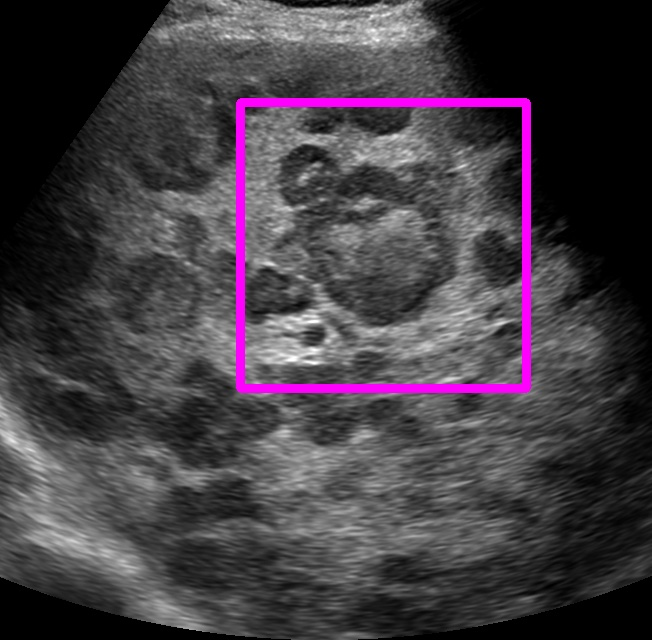
\includegraphics[width=.9\linewidth]{../fig/pseudo_a.png}
				\caption{ラベル不足のある診断画像例}
				\label{fig:ex}
			\end{minipage}
		\end{figure}

\footnotetext[1]{今回は\Fref{ex}の様なアノテーションが不足しているものを指す}
\addtocounter{footnote}{1}

	\section{これまでの研究のまとめ}
		\begin{itemize}
			\item データセット
			\begin{itemize}
				\item 国立研究開発法人日本医療研究開発機構(AMED)\footnote{\url{https://www.amed.go.jp/}}が提供している延べ8万枚に及ぶ以下のデータが付随
				\begin{itemize}
					\item 腹部超音波画像,ROI
					\item 年齢,性別
				\end{itemize}
                \begin{figure}[h]
					\centering
                    \subfloat[性別毎の画像枚数]{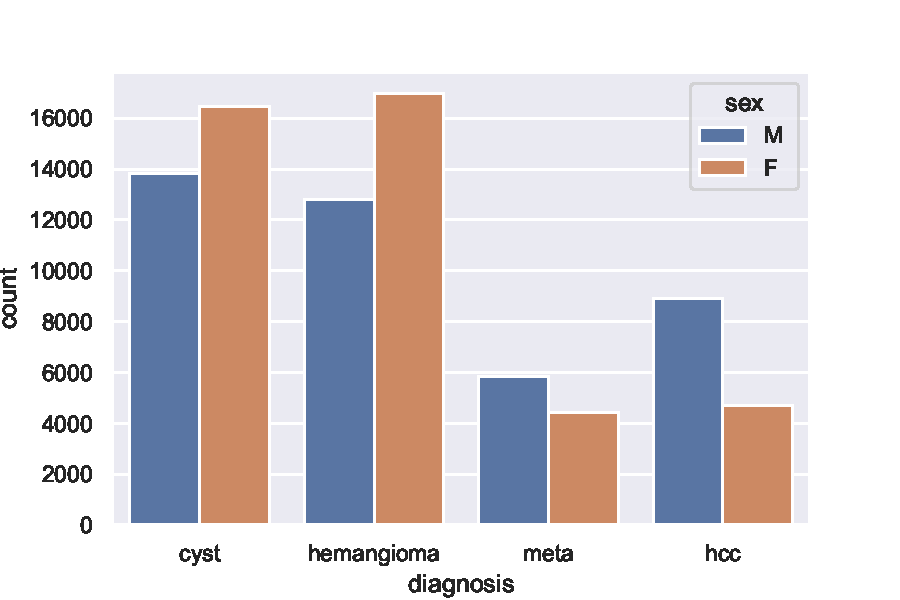
\includegraphics[width=.49\linewidth]{../fig/sex_a.pdf} \label{fig:sex}}
                    \subfloat[診断名毎の年齢分布]{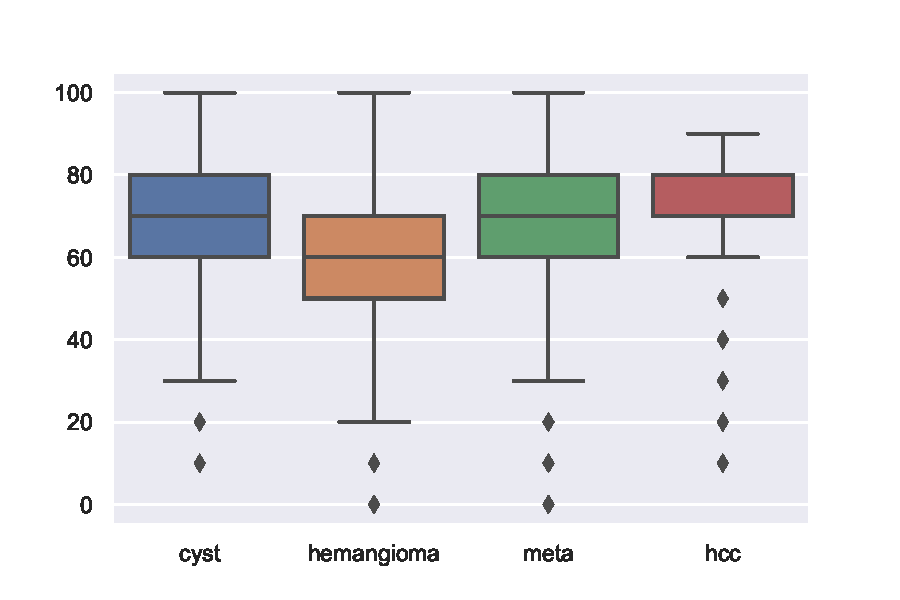
\includegraphics[width=.49\linewidth]{../fig/age_a.pdf} \label{fig:age}}
                    \caption{データセットにおけるメタデータの分布}
                \end{figure}
				\item 性別(\Fref{sex})
				\begin{itemize}
					\item hcc(肝細胞癌)は男性が罹患しやすい
					\begin{itemize}
                        \item 昔は男性の方が飲酒・タバコが多く癌に罹りやすかったという時代背景があるかもしれない
                    \end{itemize}
					\item hemangioma(血管腫)は女性が罹患しやすい
					\item meta(転移性肝癌)は他の症状よりも少ない
				\end{itemize}
				\item 年齢(\Fref{age})
				\begin{itemize}
					\item cyst(単純嚢胞),hemangioma(血管腫)の分布にははあまり特徴がない
					\item hemangioma(血管腫)は比較的若年層でも罹患する
					\item meta(転移性肝癌)における0歳はラベルミスである可能性が高い
                    \item hcc(肝細胞癌)は比較的高齢者が罹患しやすい
				\end{itemize}
                \begin{figure}[ht]
					\subfloat[診断名毎の画像サイズ$(h \times w)$の分布]{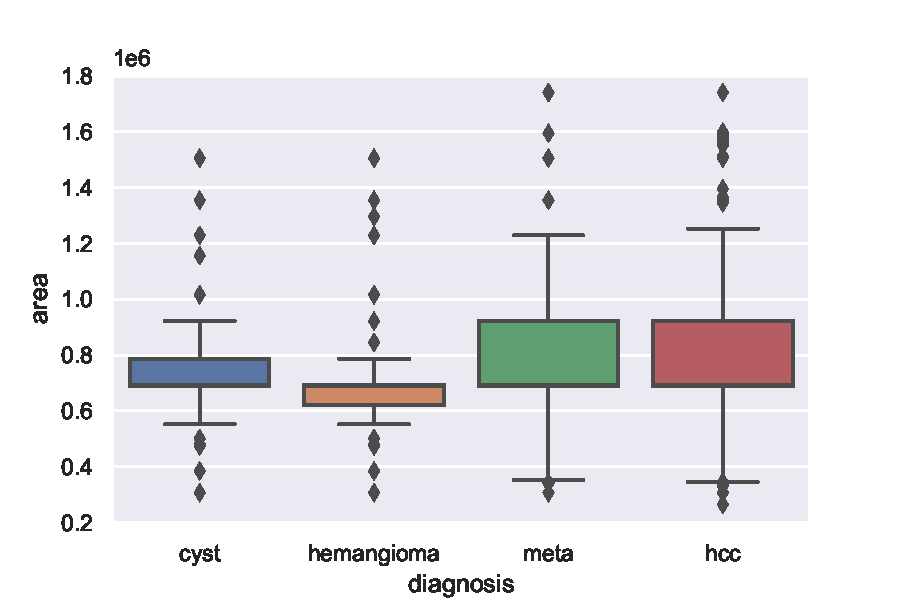
\includegraphics[width=.49\linewidth]{../fig/area_a.pdf} \label{fig:area}}
					\subfloat[診断名毎のbboxの割合]{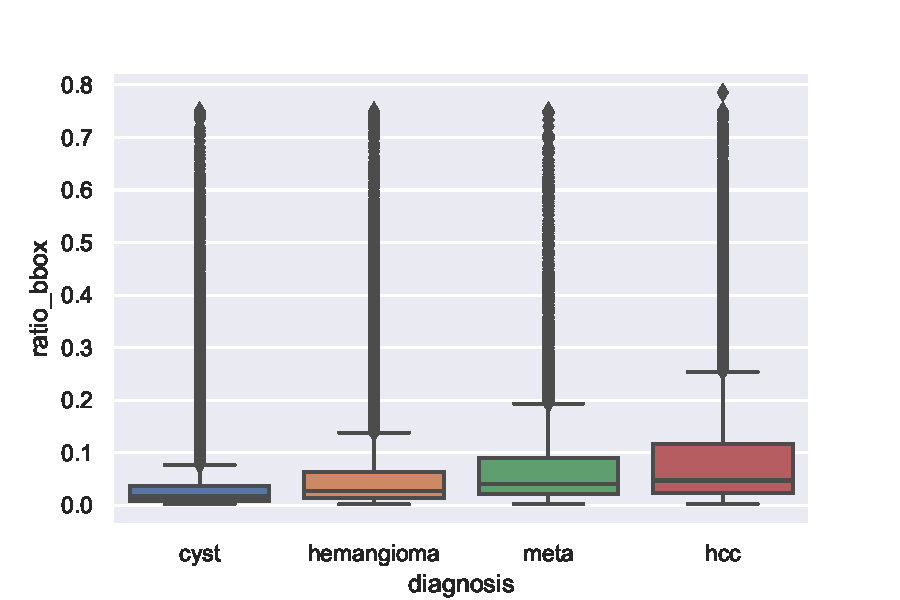
\includegraphics[width=.49\linewidth]{../fig/ratio_bbox_a.pdf} \label{fig:ratio}}
					\caption{データセットにおける画像及びbboxの割合の分布}
				\end{figure}
				\item 画像サイズ(\Fref{area})
				\begin{itemize}
                    \item hemangioma(血管腫)は比較的画像サイズが統一されている
					\begin{itemize}
                        \item 腫瘍の大きさが血管に依存するためあまり偏りが生じていない?
                    \end{itemize}
				\end{itemize}
				\item bboxの画像に占める割合(\Fref{ratio})
                \begin{itemize}
                    \item cyst(単純嚢胞)は他の診断と比べてbboxの割合が低い($\frac{1}{2}$程度)である
                    \item hcc(肝細胞癌)は画像に占めるbboxの割合が高い
                \end{itemize}
			\end{itemize}
        \end{itemize}
        \begin{itemize}
            \item データクレンジング
            \begin{figure}[ht]
				\centering
				\subfloat[クレンジング前]{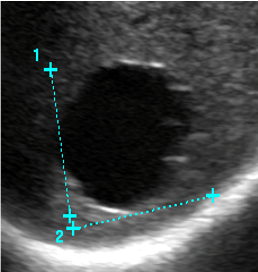
\includegraphics[width=.24\linewidth]{../fig/row.png} \label{fig:row}}
				\subfloat[マスクの生成]{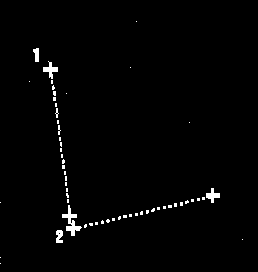
\includegraphics[width=.24\linewidth]{../fig/extract.png} \label{fig:extract}}
				\subfloat[改善前]{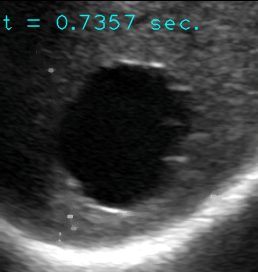
\includegraphics[width=.24\linewidth]{../fig/before.png} \label{fig:before}}
				\subfloat[改善後]{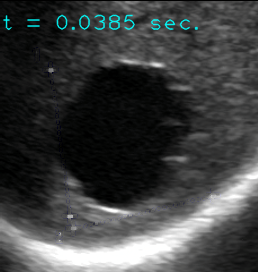
\includegraphics[width=.24\linewidth]{../fig/after.png} \label{fig:after}}
				\caption{データクレンジングを行った結果}
			\end{figure}
            \begin{enumerate}
                \item $400 \times 400$ 以下の画像の除外
				\item Perceptual Hashを利用した類似画像の除外
				\item 青色や黄色のスケールの除去
            \end{enumerate}
            \begin{itemize}
                \item \Fref{after}の様に元の精度を保ったまま約20倍高速化
            \end{itemize}
            \item 提供されているデータをCOCODatasetの形式に変換
            \begin{itemize}
                \item train data : test data : val data = 67122 : 8390 : 8391
            \end{itemize}
		\end{itemize}

\clearpage
    
    \section{前回のGMからの進捗}
        \begin{itemize}
            \item 症状毎の特徴を調査
            \begin{figure}[h]
				\centering
				\subfloat[cyst(単純嚢胞)]{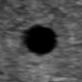
\includegraphics[width=.24\linewidth]{../fig/cyst.png} \label{fig:cyst}}
				\subfloat[hemangioma(血管腫)]{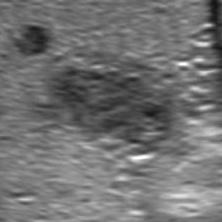
\includegraphics[width=.24\linewidth]{../fig/hemangioma.png} \label{fig:hemangioma}}
				\subfloat[meta(転移性肝癌)]{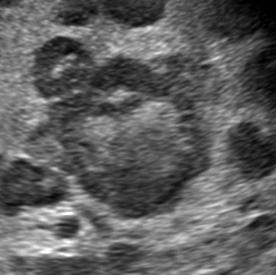
\includegraphics[width=.24\linewidth]{../fig/meta.png} \label{fig:meta}}
				\subfloat[hcc(肝細胞癌)]{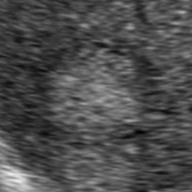
\includegraphics[width=.24\linewidth]{../fig/hcc.png} \label{fig:hcc}}
				\caption{症状毎における腫瘍の超音波画像}
			\end{figure}
            \begin{itemize}
                \item cyst(単純嚢胞) (\Fref{cyst})
                \begin{itemize}
                    \item 液体が貯留されている状態
                    \item 症状がでないことが多いため大きな腫瘍になって発見されることが多い
                    \item 嚢胞の内腔に向けて増殖するため転移することは少ない
                \end{itemize}
                \item hemangioma(血管腫) (\Fref{hemangioma})
                \begin{itemize}
                    \item 肝臓にできる良性腫瘍の中で最も多い
                    \item 女性ホルモンが原因で女性が罹患しやすいと言われているが詳しくは解明されていない
                    \item 血管が無数に絡み合うことによって出来た血管の塊であることから血流が遅いという特徴がある
                    \item 他の臓器に浸潤したり転移することは無いと言われている
                \end{itemize}
                \item meta(転移性肝癌) (\Fref{meta})
                \begin{itemize}
                    \item 門脈を介して大腸癌などの消化器癌から転移する割合が多い
                    \item 類似したエコーパターンをもつ腫瘤が多発してみられることが多い
                \end{itemize}
                \item hcc(肝細胞癌) (\Fref{hcc})
                \begin{itemize}
                    \item 肝臓にできる悪性腫瘍の中で最も多いと言われている
                    \item 約90%がウイルス感染症が原因
                    \begin{itemize}
                        \item B型肝炎ウイルス(HBV)が約20\%
                        \item C型肝炎ウイルス(HCV)が約70\%
                    \end{itemize}
                \end{itemize}
            \end{itemize}
            \item YOLOXを用いた4クラスの腫瘍検出
            \begin{itemize}
                \item 学習条件
            \end{itemize}
            \begin{minipage}{.95\textwidth}
                \stackunder{
                    \begin{minipage}[h]{.44\textwidth}
                        \setcounter{table}{0}
                        \centering
                        \label{tab:conditions}
                        \begin{tabular}{c|c}
                            seed & 0 \\
                            model & YOLOX-s \\
                            pretrained & ImageNet \\ \hline
                            data数 & 67122 \\
                            batch\_size & 64 \\
                            total\_epoch & 50 \\
                            input\_size & (512, 512) \\ \hline
                            weight\_decay & 0.0005 \\
                            momentum & 0.9 \\
                            scheduler & yoloxwarmcos \\
                            criterion & BCELoss \\ \hline
                            device & gpgpu8 \\
                            計算時間 & 30 min/epoch \\
                        \end{tabular}
                    \end{minipage}
                }
                {
                    \begin{minipage}[h]{.44\textwidth}
                        \captionof{table}{学習に用いた条件}
                    \end{minipage}
                }
                \hfill
                \stackunder{
                    \begin{minipage}[h]{.54\textwidth}
                        \centering
                        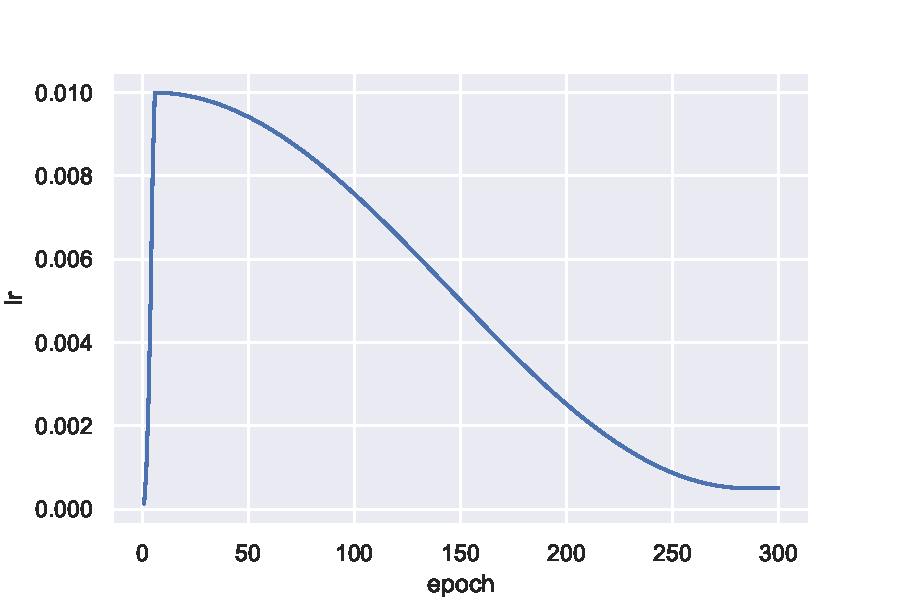
\includegraphics[width=\linewidth]{../fig/yoloxs_lr.pdf}
                    \end{minipage}
                }
                {
                    \begin{minipage}[h]{.54\textwidth}
                        \setcounter{figure}{6}
                        \captionof{figure}{yoloxwarmcos}
                    \end{minipage}
                }
            \end{minipage}

\clearpage

            \begin{itemize}
                \item 学習結果
                \begin{figure}[h]
                    \centering
                    \subfloat[AP]{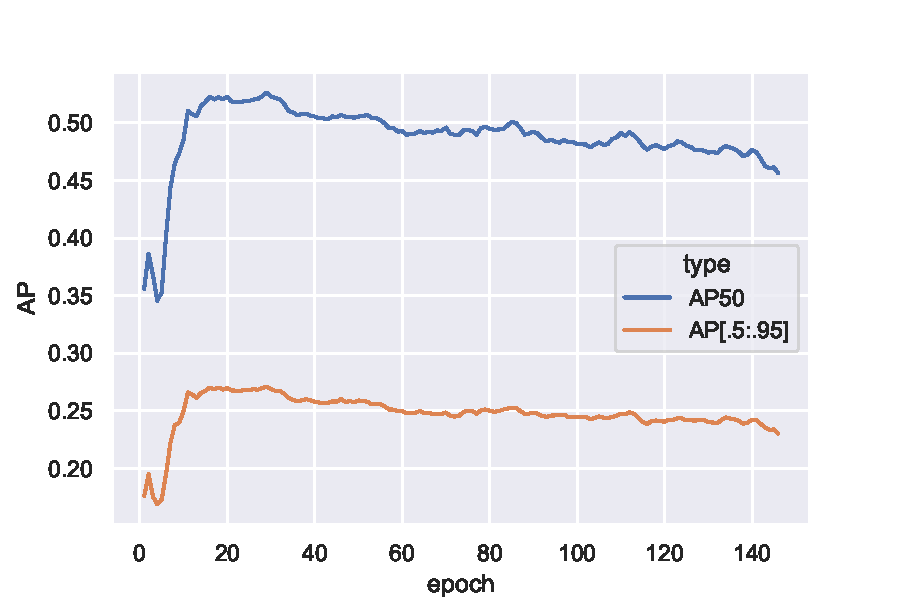
\includegraphics[width=.49\linewidth]{../fig/yoloxs4_AP.pdf} \label{fig:ap}}
                    \subfloat[loss]{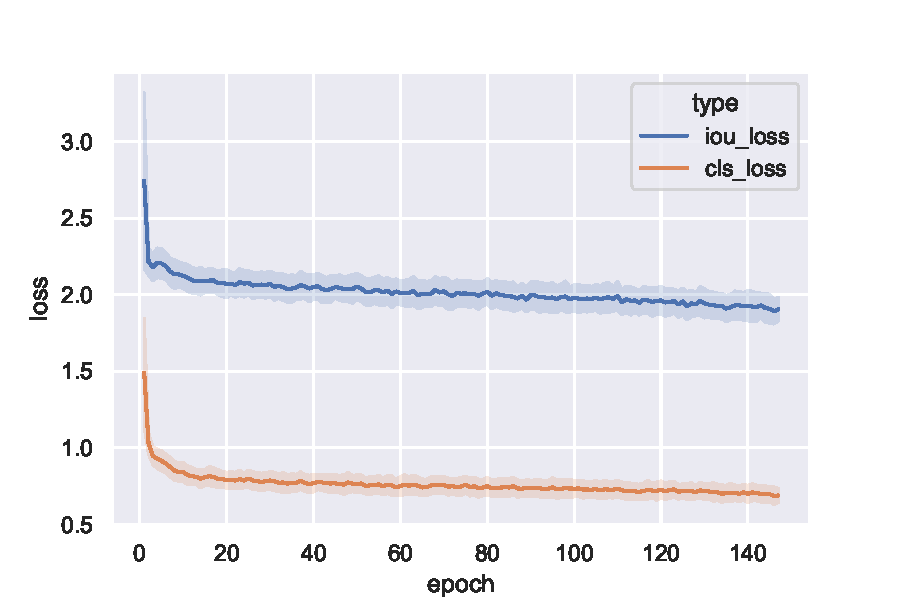
\includegraphics[width=.49\linewidth]{../fig/yoloxs4_loss.pdf} \label{fig:loss}}
                    \caption{YOLOXで4クラスの検出を行った時のAPとloss}
                \end{figure}
                \item 考察
                \begin{itemize}
                    \item クラスを誤って検出しているものが多い可能性がある
                \end{itemize}
                \end{itemize}
                \item YOLOXを用いた1クラスでの腫瘍検出
                \begin{itemize}
                    \item 学習条件
                    \begin{itemize}
                        \item ほぼ\Tref{conditions}と同様
                        \item total\_epoch = 300
                    \end{itemize}
                    \item 学習結果
                    \begin{figure}[h]
                        \centering
                        \subfloat[AP]{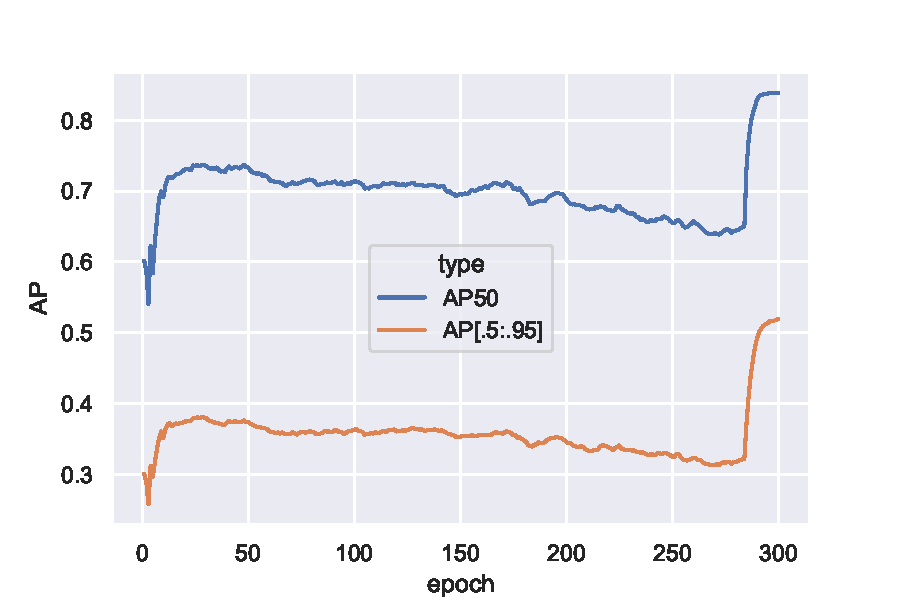
\includegraphics[width=.49\linewidth]{../fig/yoloxs1_AP.pdf} \label{fig:ap}}
                        \subfloat[loss]{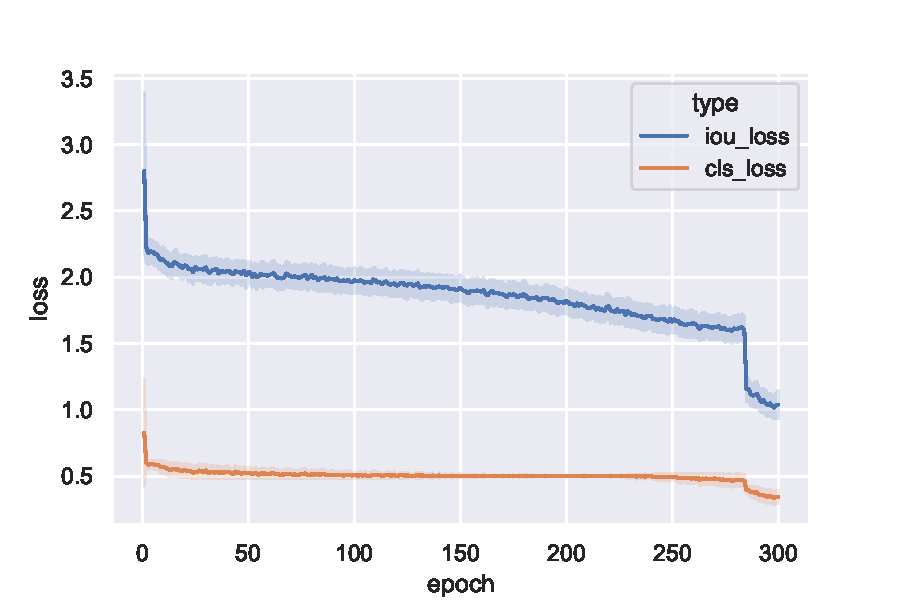
\includegraphics[width=.49\linewidth]{../fig/yoloxs1_loss.pdf} \label{fig:loss}}
                        \caption{YOLOXで1クラスの検出を行った時のAPとloss}
                    \end{figure}
                \end{itemize}
                \begin{itemize}
                    \item 考察
                    \begin{itemize}
                        \item Double Descentが起きている?
                        \item Noisy Labelが最も大きな要因らしい
                    \end{itemize}
                \end{itemize}

\clearpage

                \item まとめ
                \begin{figure}[h]
                    \centering
                    \subfloat[mAP]{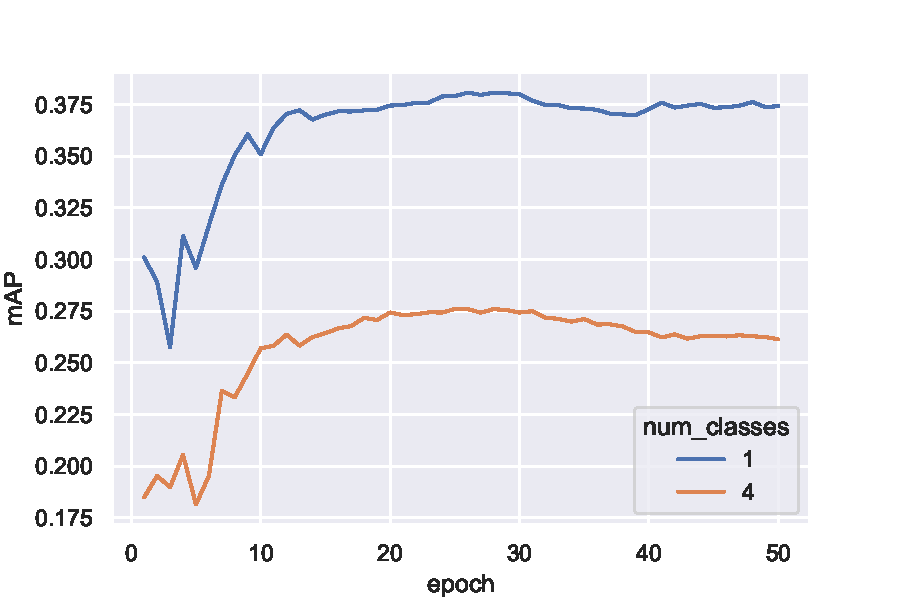
\includegraphics[width=.32\linewidth]{../fig/compare_mAP.pdf} \label{fig:ap}}
                    \subfloat[iou\_loss]{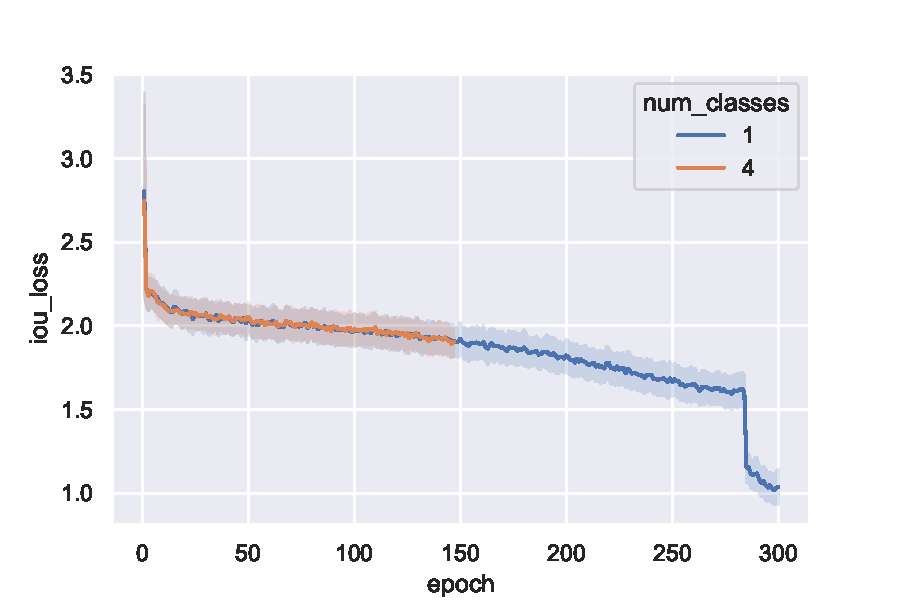
\includegraphics[width=.32\linewidth]{../fig/compare_iou_loss.pdf} \label{fig:iou_loss}}
                    \subfloat[cls\_loss]{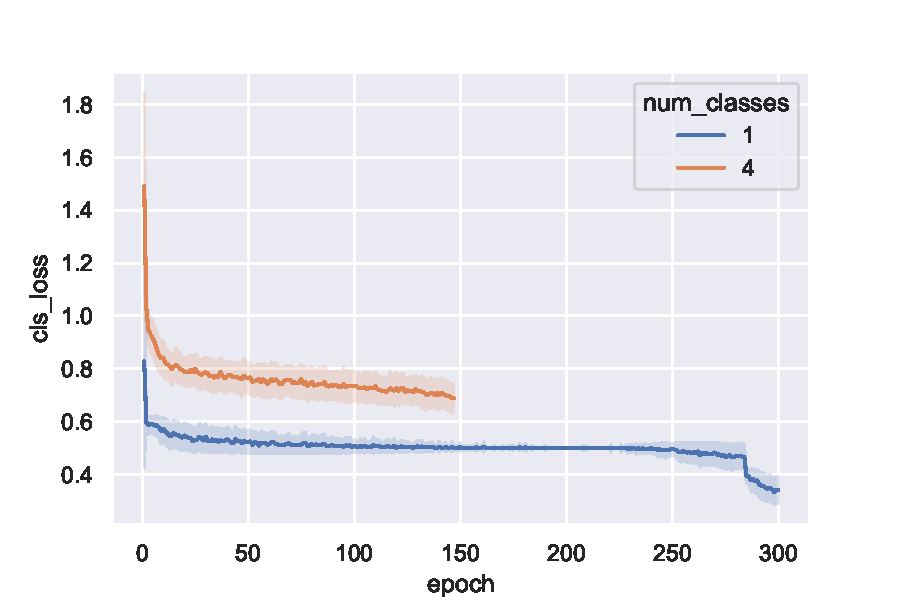
\includegraphics[width=.32\linewidth]{../fig/compare_cls_loss.pdf} \label{fig:cls_loss}}
                    \caption{YOLOXで腫瘍検出を行った際のクラス数によるAPとlossの比較}
                \end{figure}
                \begin{table}[h]
                    \centering
                    \caption{学習で得られた精度}
                    \label{tab:exp}
                    \begin{tabular}{ccc|ccc|ccc}
                            & & & & IoU & & & area \footnotemark & \\
                        model & backbone & num\_classes & mAP & AP$_{50}$ & AP$_{75}$ & AP$_S$ & AP$_M$ & AP$_L$ \\ \hline
                        \multirow{2}{*}{YOLOX\cite{yolox}} & \multirow{2}{*}{Decoupled head} & 1 & 0.519 & 0.839 & 0.558 & - & 0.639 & 0.631 \\
                            &  & 4 & 0.277 & 0.531 & 0.256 & - & 0.215 & 0.294 \\
                    \end{tabular}
                \end{table}
                \begin{itemize}
                    \item 考察
                    \begin{itemize}
                        \item mAPが25\%程度向上している
                        \item iou\_lossは1・4クラスの検出ともに変化なし
                        \item cls\_lossは1クラスの方が極端に低い値となっている
                        \begin{itemize}
                            \item クラス分類をしていないから当たり前
                        \end{itemize}
                        \item 1クラスの検出ではAP$_M$に比べてAP$_L$の方が小さい値となっている
                        \begin{itemize}
                            \item 4クラスでの検出に比べてbboxが小さ目に出力されている?
                        \end{itemize}
                    \end{itemize}
                \end{itemize}
            \end{itemize}
        \footnotetext{Small $< 32^2 <$ Medium $<96^2<$ Large}
    
    \section{今後の課題\&スケジュール}
        \begin{itemize}
            \item 12月半ばまでに
            \begin{itemize}
                \item 1クラス
                \begin{itemize}
                    \item PR曲線
                \end{itemize}
                \item 4クラス
                \begin{itemize}
                    \item PR曲線
                    \item 腫瘍の種類毎の再現率・適合率
                \end{itemize}
            \end{itemize}
            \item できるだけ早めに
            \begin{itemize}
                \item 研究の方向性を決める
                \item Confident Learning \cite{cleanlab} を利用してみる
                \begin{itemize}
                    \item ラベルにノイズが含まれていると予想されるデータセットに対して精度を向上させることができる
                    \item pipでインストールできるcleanlab\footnote{\url{https://github.com/cleanlab/cleanlab}}というライブラリを用いることで簡単に使える
                    \begin{itemize}
                        \item 調べてみたら元はKeras?
                    \end{itemize}
				\end{itemize}
            \end{itemize}
        \end{itemize}

        \begin{thebibliography}{9}
            \bibitem{yolox} Zheng Ge, Songtao Liu, Feng Wang, Zeming Li, and Jian Sun. \href{https://arxiv.org/pdf/2107.08430.pdf}{YOLOX: Exceeding YOLO Series in 2021}, 2021.
            \bibitem{cleanlab} Curtis G. Northcutt, Lu Jiang, and Isaac L. Chuang. \href{https://arxiv.org/pdf/1911.00068.pdf}{Confident Learning: Estimating Uncertainty in Dataset Labels}, 2021.
        \end{thebibliography}

        \clearpage

        \appendix
        \def\thesection{付録\Alph{section}}
        \section{4クラスの腫瘍検出モデルによる推論結果}
            \begin{figure}[h]
                \centering
                \subfloat[cystのラベル]{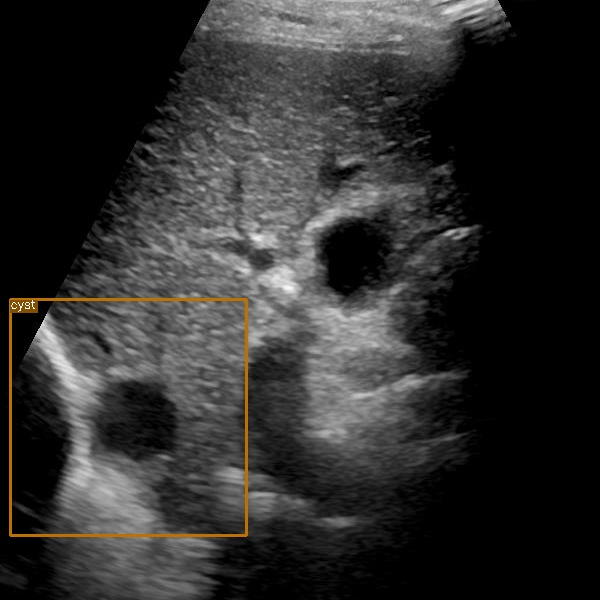
\includegraphics[width=.22\linewidth]{../fig/labeled_cyst.png} \label{fig:labeled_cyst}}
                \subfloat[hemangiomaの推論結果]{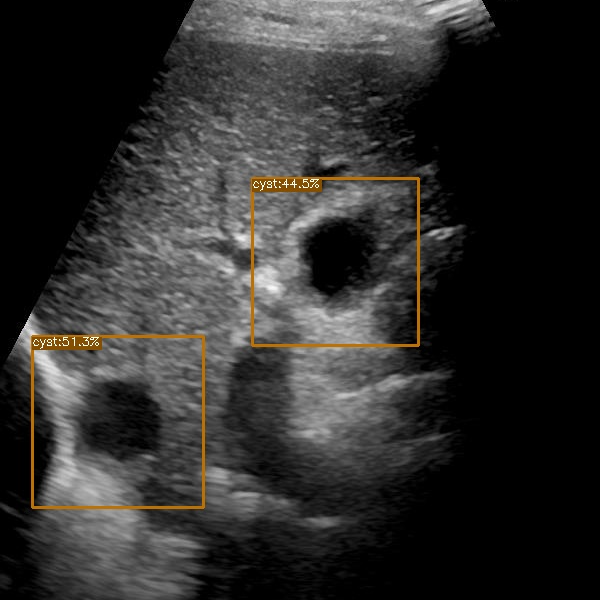
\includegraphics[width=.22\linewidth]{../fig/pred_cyst.png} \label{fig:pred_cyst}}
                \subfloat[cystのラベル]{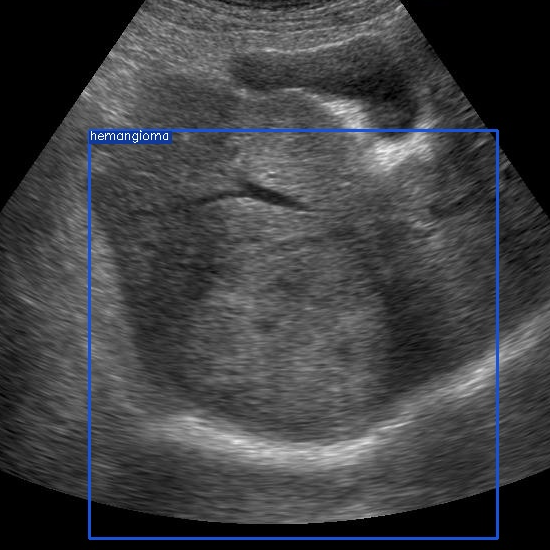
\includegraphics[width=.22\linewidth]{../fig/labeled_hemangioma.png} \label{fig:labeled_hemangioma}}
                \subfloat[hemangiomaの推論結果]{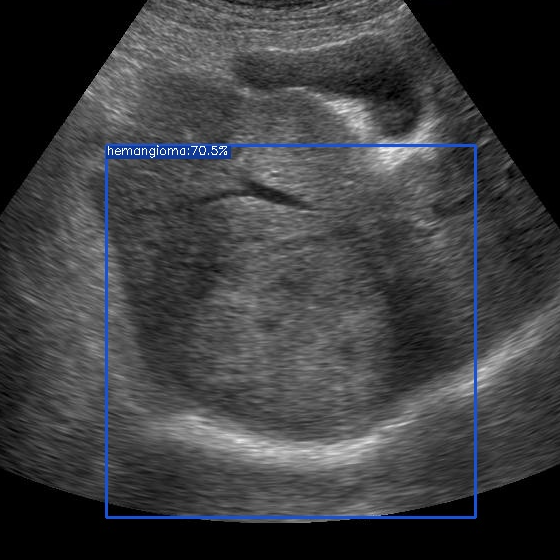
\includegraphics[width=.22\linewidth]{../fig/pred_hemangioma.png} \label{fig:pred_hemangioma}}

                \subfloat[metaのラベル]{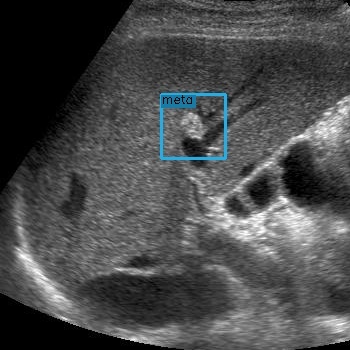
\includegraphics[width=.22\linewidth]{../fig/labeled_meta.png} \label{fig:labeled_meta}}
                \subfloat[metaの推論結果]{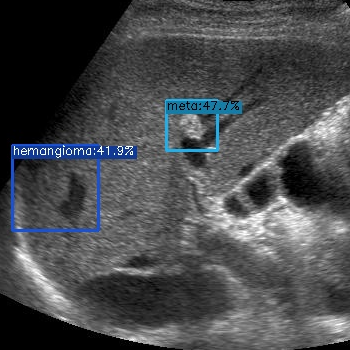
\includegraphics[width=.22\linewidth]{../fig/pred_meta.png} \label{fig:pred_meta}}
                \subfloat[hccのラベル]{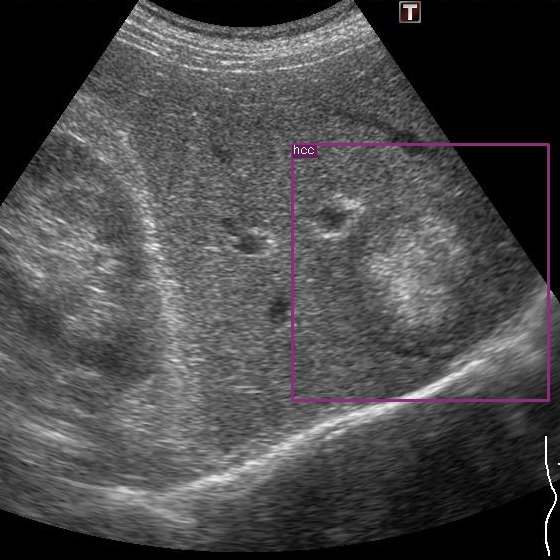
\includegraphics[width=.22\linewidth]{../fig/lebeled_hcc.png} \label{fig:labeled_hcc}}
                \subfloat[hccの推論結果]{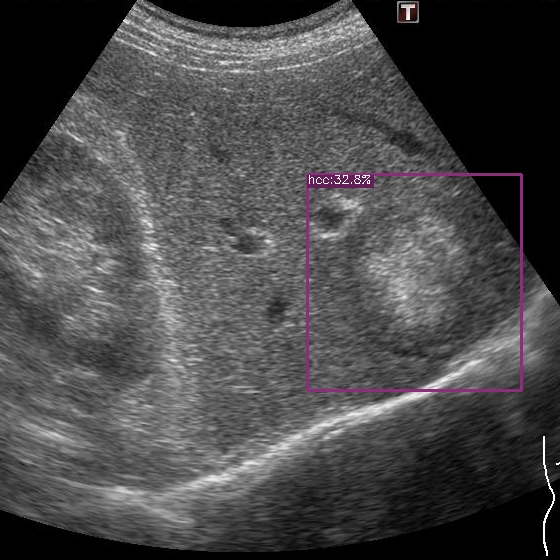
\includegraphics[width=.22\linewidth]{../fig/pred_hcc.png} \label{fig:pred_hcc}}
                \caption{画像に付随しているラベルとその正しい推論結果}
            % \end{figure}
            % \begin{figure}[h]
                \centering
                \subfloat[cystのラベル]{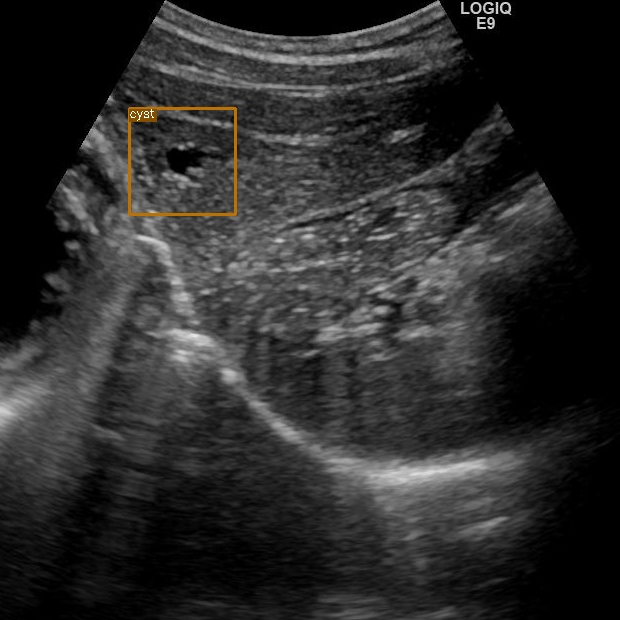
\includegraphics[width=.22\linewidth]{../fig/labeled_error_cyst.png} \label{fig:labeled_error_cyst}}
                \subfloat[cystの推論結果]{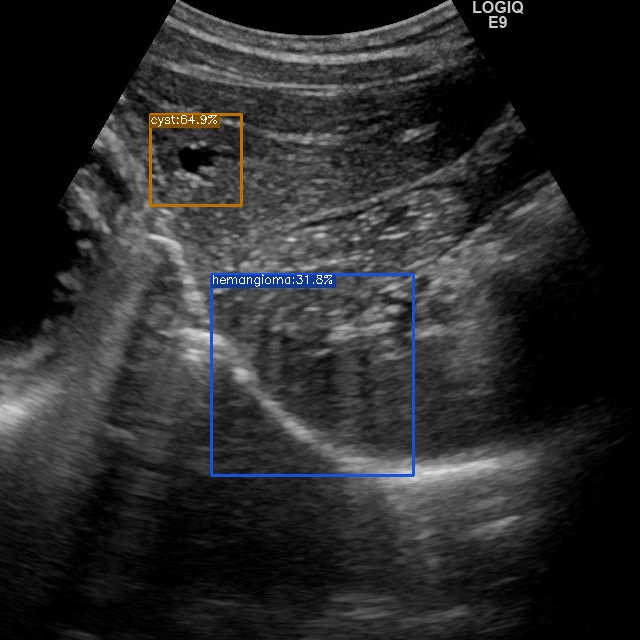
\includegraphics[width=.22\linewidth]{../fig/pred_error_cyst.png} \label{fig:pred_error_cyst}}
                \subfloat[metaのラベル]{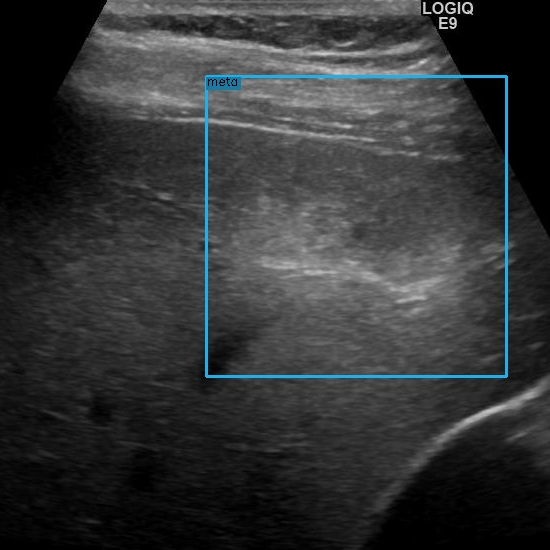
\includegraphics[width=.22\linewidth]{../fig/labeled_error_meta.png} \label{fig:labeled_error_meta}}
                \subfloat[metaの推論結果]{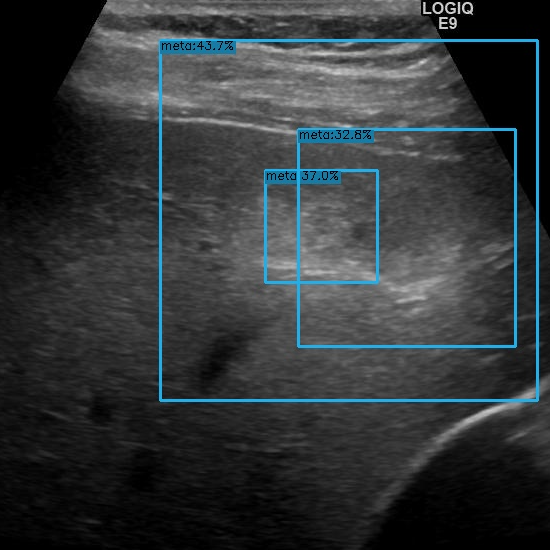
\includegraphics[width=.22\linewidth]{../fig/pred_error_meta.png} \label{fig:pred_error_meta}}

                \subfloat[hemangiomaのラベル]{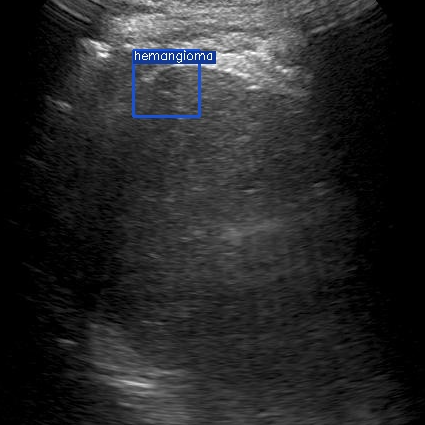
\includegraphics[width=.22\linewidth]{../fig/labeled_error_hemangioma.png} \label{fig:labeled_error_hemangioma}}
                \subfloat[hemangiomaの推論結果]{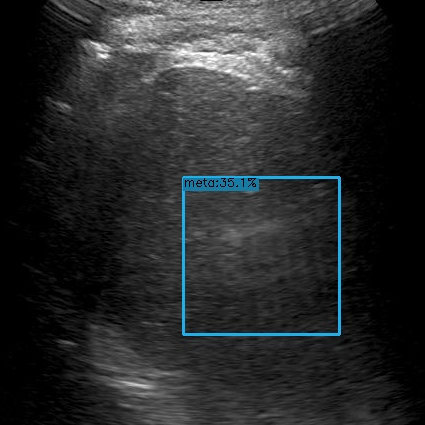
\includegraphics[width=.22\linewidth]{../fig/pred_error_hemangioma.png} \label{fig:pred_error_hemangioma}}
                \subfloat[hccのラベル]{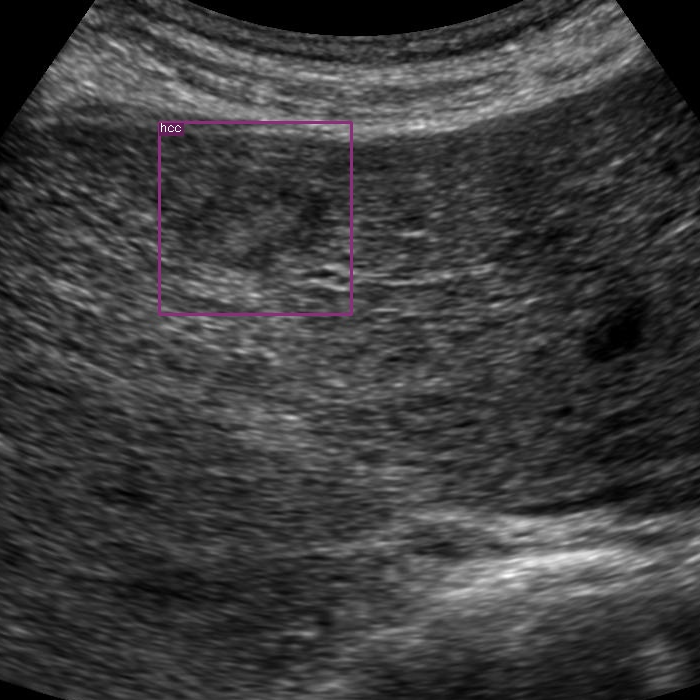
\includegraphics[width=.22\linewidth]{../fig/labeled_error_hcc.png} \label{fig:labeled_error_hcc}}
                \subfloat[hccの推論結果]{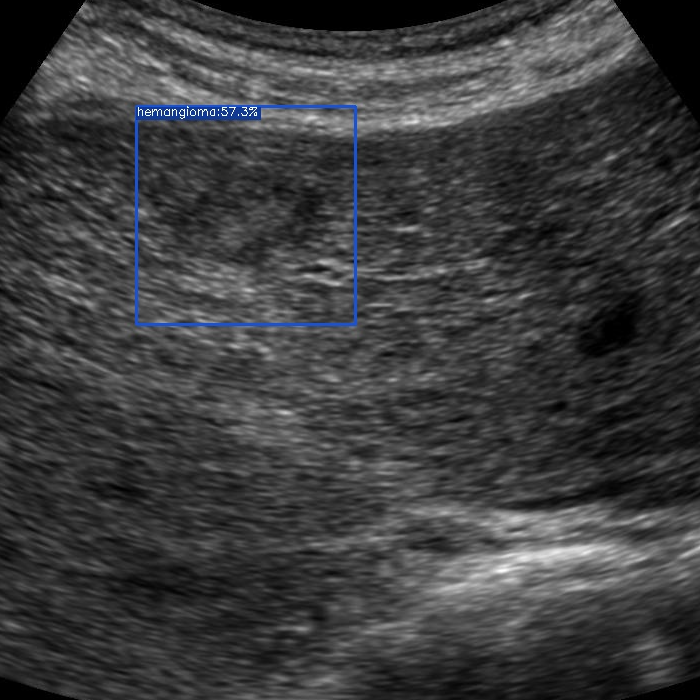
\includegraphics[width=.22\linewidth]{../fig/pred_error_hcc.png} \label{fig:pred_error_hcc}}
                \caption{画像に付随しているラベルとその誤った推論結果}
            \end{figure}
\end{document}
